\section{Self Study 2: Database Modeling}
\deadline{12}{3}{2014}

\subsection{Entity-relationship Diagram}
In figure \ref{fig:ss2-ERdiagram}, we show an updated ER diagram based on concepts we've learned in the course.
\begin{figure}[h]
  \centering
  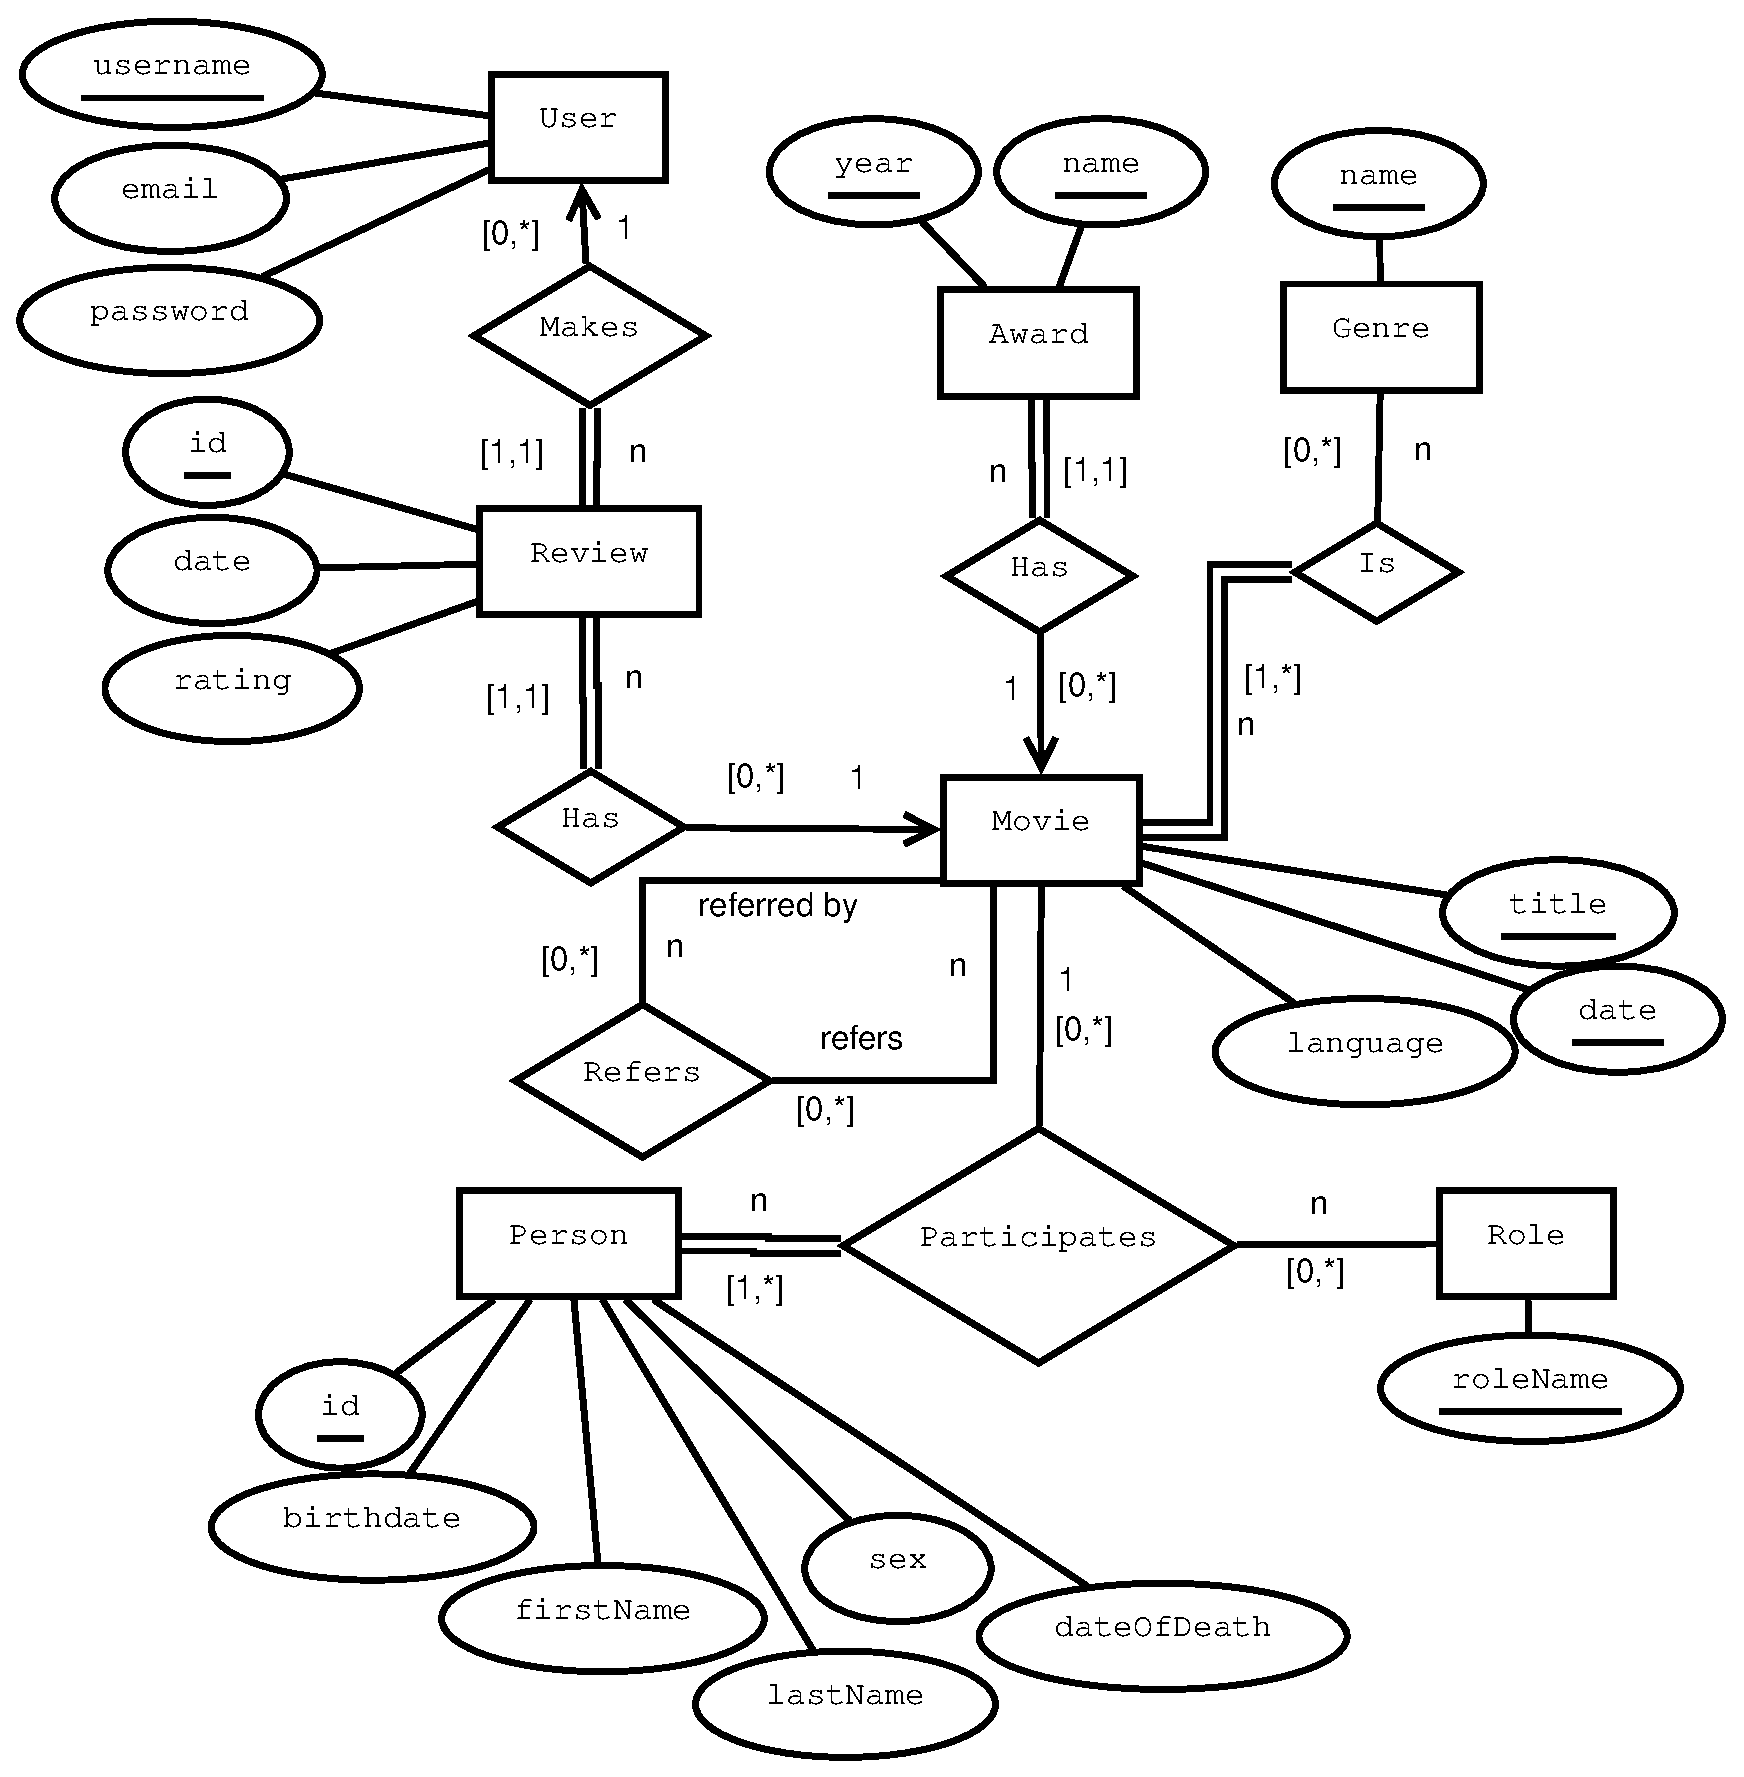
\includegraphics[width=\linewidth]{2-17.02.14/ERDiagram.eps}
  \caption{ER diagram of an IMDB-like website.}\label{fig:ss2-ERdiagram}
\end{figure}

Primary keys are underlined. Chen, min max, and arrows on lines represent the different cardinalities between entities and their relations. Circles are attributes and squares represent entities. Diamonds are relationships, just like we have learned in the course. 

\subsection{Schema}
The entities and relationships have been mapped to relations in the diagram of figure \ref{fig:ss2-schema}.
\begin{figure}[h]
  \centering
  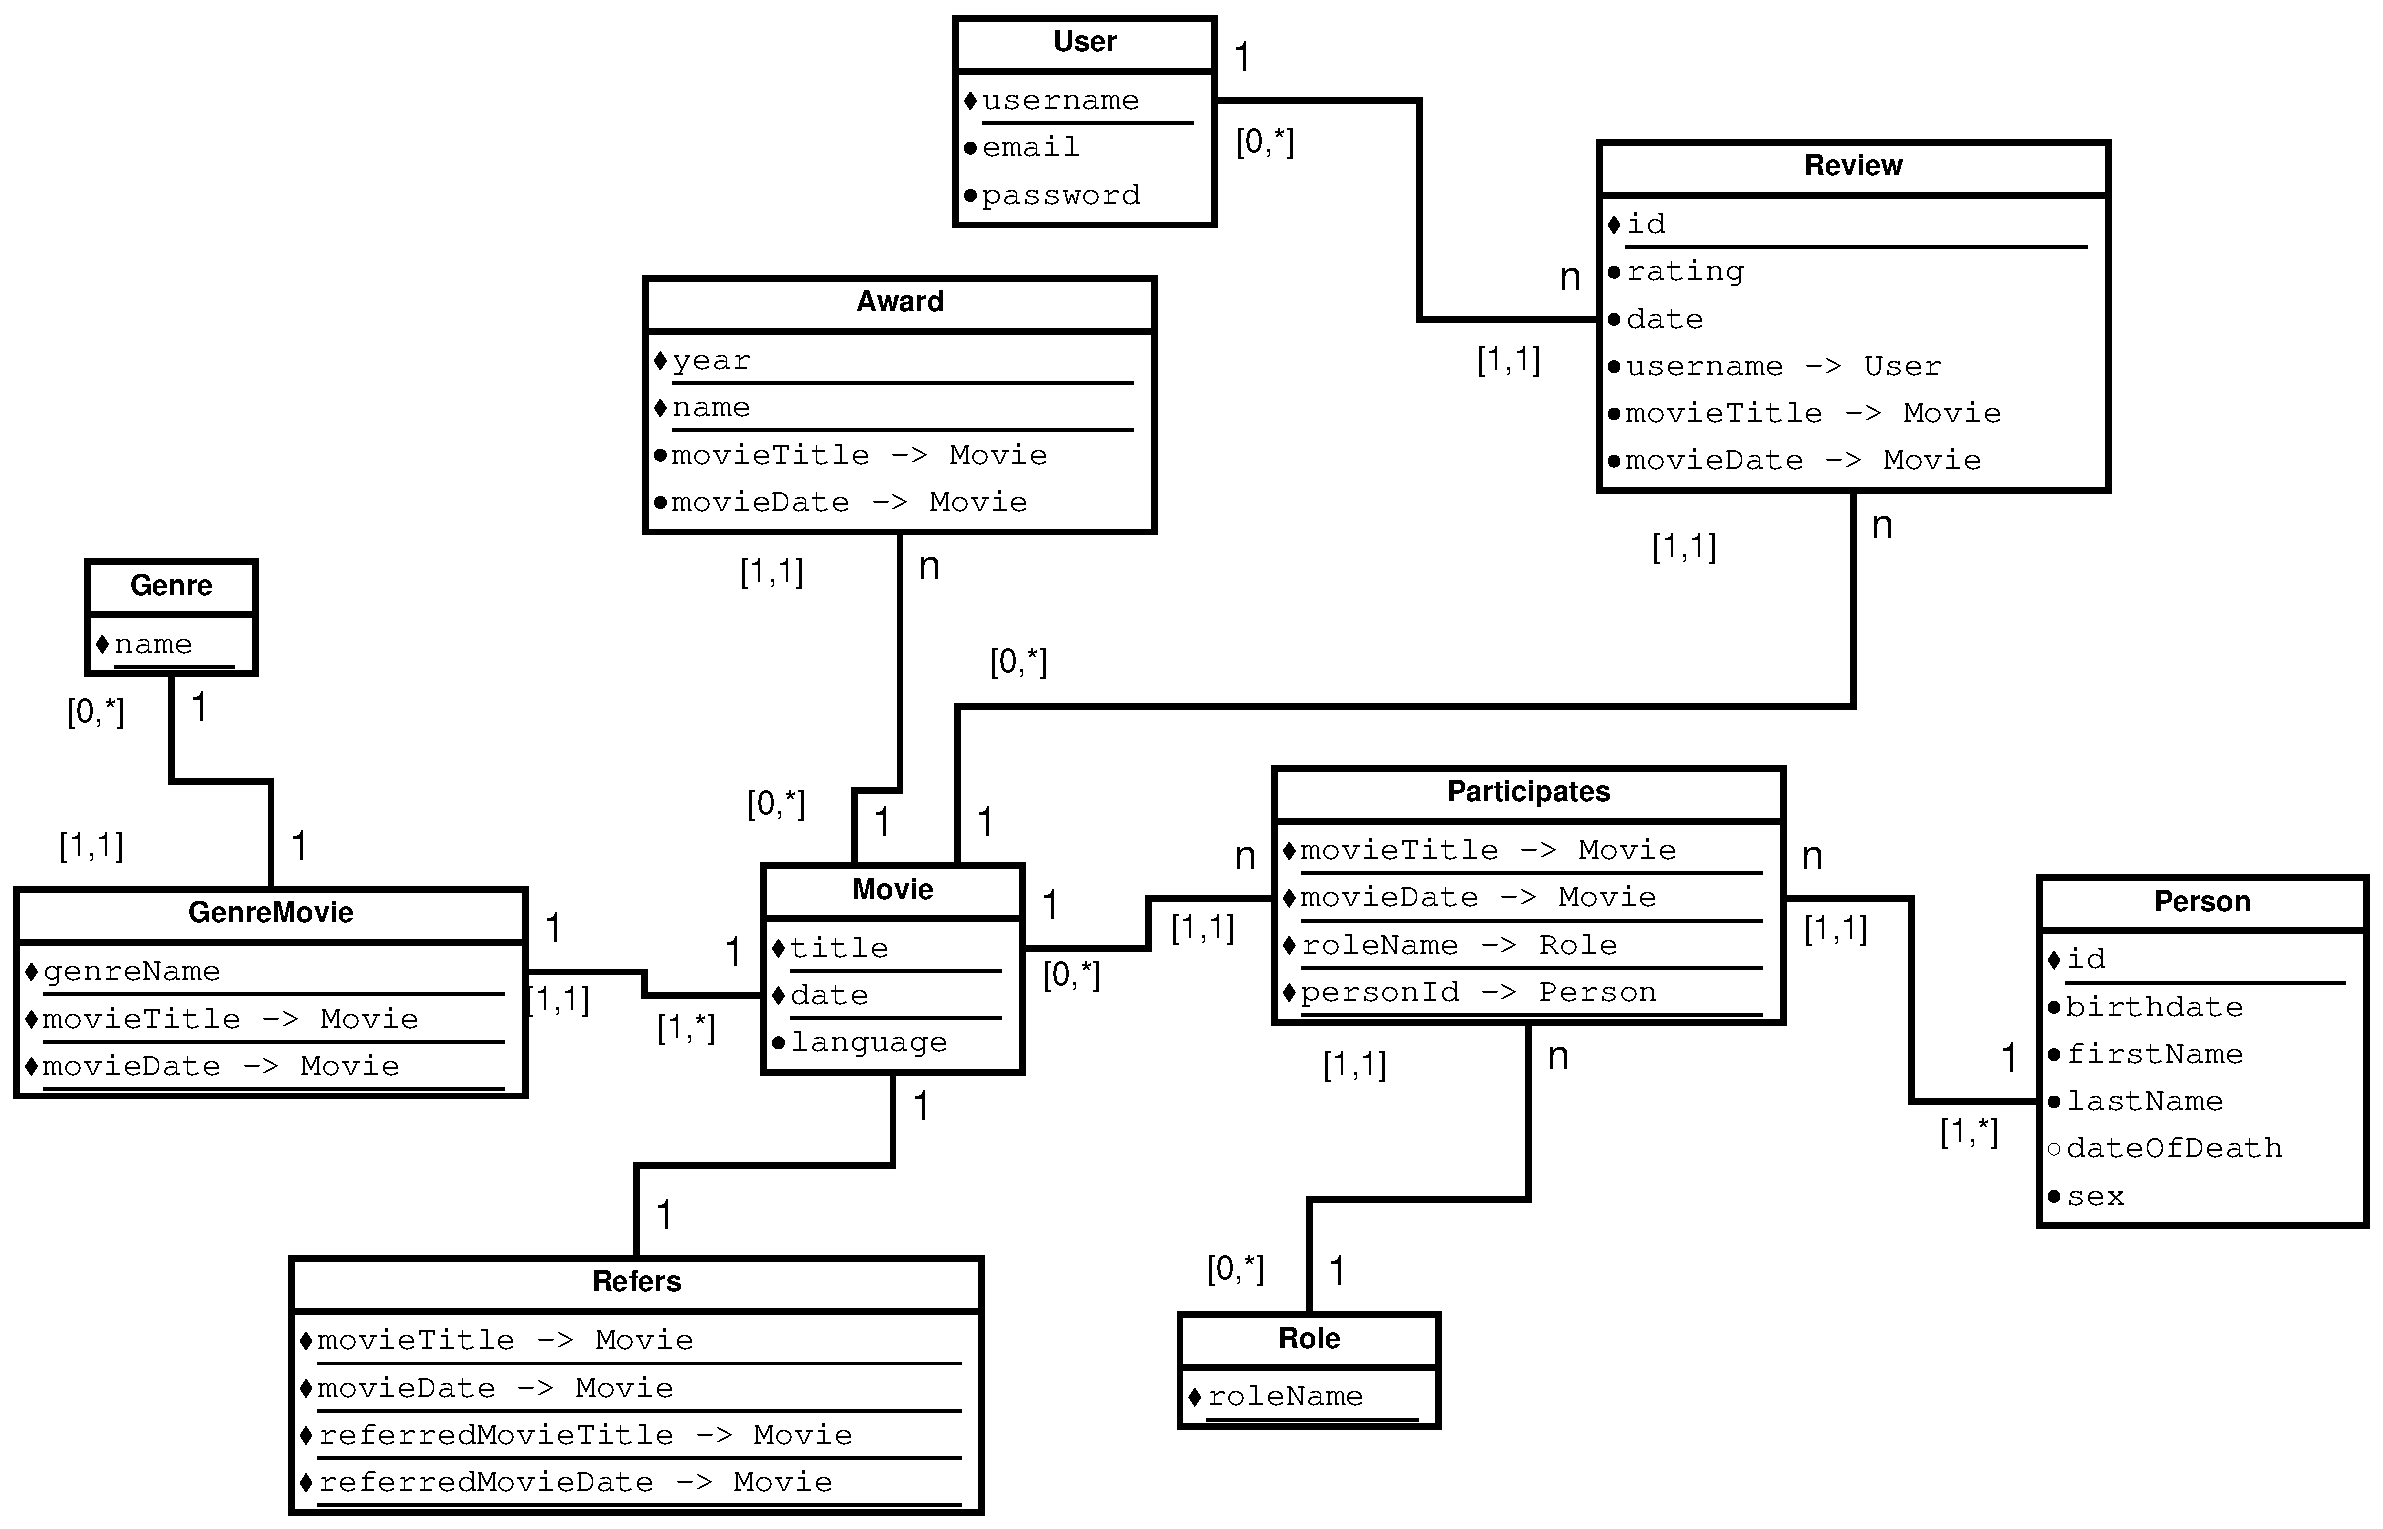
\includegraphics[width=\linewidth]{2-17.02.14/DatabaseSchema.eps}
  \caption{The schema, i.e.\ mapped relations of an IMDB-like website.}\label{fig:ss2-schema}
\end{figure}
Attributes acting as foreign keys in relation $A$ are marked by an ASCII arrow \texttt{->}, where the arrow points to the primary key(s) in relation $B$. The symbols to the left of each attribute signal whether the attribute can be null or not. When black, they cannot take on the null value, when hollow, the attribute can be null, like the \emph{dateOfDeath} attribute on the \emph{Person} relation, since we cannot know when living actors/directors will die.

\subsection{Non-trivial considerations}
The \emph{Participate} relationship is 3-way due to the fact that many \emph{People} (actors) can have many different roles in different movies, or even multiple roles in one movie. This relationship construct allows us to express both in the database.

\subsection{Comparison of the previous and current solution}

In our first attempt to construct a diagram for the movie database, we used the Enhanced Entity-Relationship (EER) model to construct the relevant information for the database.
In this version of our database, we use the Entity-Relationship (ER) model as described in the course.

In this version we include Chen notation and min-max notation to emphasize to type of relations. 
This is also visualised in form of arrows or no arrows on each connection between relations.
Another clear difference is that we include total participation for some of the relations.
Actually, total and partial participation is expressed as identifying and non-identifying relations in the EER model. This is not covered in the course.
We could also have included weak entities, but we did not find any which should be marked as weak. 

We have removed redundancy, because an actor can also be a director in movies.
We have introduced a relation called Role in which it is clear which role a person has in a given movie.
We also considered an ISA relation between the roles in a movie.
We chose not to use it, because there is nothing different between an actor and a director.

We have only included the necessary primary keys. 
If there was no need for a unique id, we have not included one.

